\documentclass[xcolor={dvipsnames,table}]{beamer}
\mode<presentation>{\usetheme{Warsaw}\usecolortheme{crane}}
\usepackage{centernot}
\usepackage{graphicx}
\usepackage{geometry}
\usepackage{tikz}
\usetikzlibrary{shadows}

\usefonttheme{serif}
\usepackage[utf8]{inputenc}
\usepackage[english]{babel}
\usepackage{lmodern}
\usepackage[T1]{fontenc}
\usepackage[babel=true]{microtype}

\title{UNIX Weapons School---Computer Architecture}
\date{}
\author{Nick Black for the\\
Georgia Institute of Technology
}

\begin{document}

\begin{frame}
\titlepage
\begin{center}

\includegraphics[scale=0.33]{images/uws.png}\\
\vspace{.1in}
\tiny{copyright \copyright\ 2013}\\

\includegraphics[scale=.25]{images/cc-logo.pdf}

\includegraphics[scale=.25]{images/cc-new.pdf}

\includegraphics[scale=.25]{images/cc-share.pdf}\\
\tiny{creative commons 3.0 share-alike attribution license}
\end{center}
\end{frame}

\begin{frame}{Recommended reading}
\small
\begin{itemize}
\item Andi Kleen. ``Linux multi-core scalability'' (2009).
\item Doug Carmean and Eric Sprangle. ``Increasing Processor Performance by Implementing Deeper Pipelines'' (2002).
\item Ulrich Drepper. ``What Every Programmer Needs to Know About Memory'' (2007). Linux Weekly News, in eight parts.
\item Paul McKenney. ``Transactional Memory Everywhere'' (2012).
\item John Shen and Mikko Lipasti. \textit{Modern Processor Design} (2004).
\item Agner Fog. \textit{The microarchitecture of Intel, AMD and VIA CPUs: An optimization guide for assembly programmers and compiler makers} (regularly updated). http://www.agner.org.
\item Bruce Shriver and Bennett Smith. \textit{The Anatomy of a High-Performance Microprocessor: A Systems Perspective} (1998).
\item \textit{Intel 64 and IA-32 Architectures Optimization Manuals}.
\end{itemize}
\end{frame}

\begin{frame}{The purpose of a systems programmer}
\textbf{Given system $S$, and problem $P$,\\
we will implement $P$,\\
using the resources of $S$,\\
subject to some constraint.}\\
\vspace{.25in}
That constraint is typically to minimize either:
\begin{itemize}
\vspace{.05in}
\item time to completion,
\vspace{.05in}
\item power to completion, or
\vspace{.05in}
\item $\text{time to completion}\cdot\text{utilization.}\footnote{Constrained by some minimum utilization.}$
\end{itemize}
\vspace{.25in}
Proving that these constraints have been met is clearly
dependent upon the details of both $P$ and $S$.
\end{frame}

\begin{frame}{Chasing peak}
How can we know when we're ``done''? Absolute measurements
can be taken in terms of the system's theoretical \textbf{peak} perf.\\
\vspace{.15in}
Peak is a slippery concept. What follows are my opinions:
\vspace{.15in}
\begin{itemize}
\item ``Peak'' seems most \textit{precisely} defined in terms of the ISA of $S$
(which might be irrelevant to our problem).
\item ``Peak'' seems most \textit{correctly} defined in terms of the best possible
solution to $P$ (which might be unknown).
\item ``Peak'' seems most \textit{productively} defined in terms of the instructions our actual
implementation would use in the absence of structural hazards.
\end{itemize}
\vspace{.15in}
In my experience, it is generally misleading to compare how closely
different $P$ approach their own peaks. Most often, we use ``peak'' within
the context of a small section of code.
\end{frame}

\begin{frame}{Abstractions defrocked}
\begin{itemize}
\item ``The purpose of abstraction is not to be vague, but to create a new semantic level in which one can be absolutely precise.''\\
\hfill--Edsger Dijkstra
\vfill
\item ``First you learn the value of abstraction. Then you learn the cost of abstraction. Then you're ready to engineer.''\\
\hfill--Kent Beck
\vfill
\item We will draw the line at the electric level.
\end{itemize}
\end{frame}

\begin{frame}{Complementary metal-oxide semiconductors I}
Draw \textit{greatest} power only when changing state\ldots
\begin{equation}
P_{dynamic} = \alpha C_LV_{DD}^{2}\nu
\end{equation}
\begin{description}
\item[$P$] Dynamic power ($W = J/s = \frac{m^{2}\cdot kg}{s^{3}}$)
\item[$C_L$] Load capacitances ($F = \frac{A^{2}\cdot s^{4}}{m^{2}\cdot kg}$)
\item[$\alpha$] Activity factor
\item[$V_{DD}$] Supply voltage ($V = \frac{m^{2}\cdot kg}{A\cdot s^{3}}$)
\item[$\nu$] Frequency ($1/s$)
\end{description}
\vfill
\textbf{NB:} $P_{dynamic}$ increases with the \textit{square} of $V_{DD}$.
\end{frame}

\begin{frame}{Complementary metal-oxide semiconductors II}
\ldots but always consume \textit{some} power:
\begin{equation}
P_{static} = I_{static}\cdot V_{DD}
\end{equation}
\begin{description}
\item[$P$] Static power ($W = V\cdot A$)
\item[$I_{static}$] Static current ($I_{subth}\footnote{Leakage between MOS source and drain} + I_{tunnel}\footnote{Leakage across semiconductor junctions} + I_{leakage}\footnote{Leakage through the insulator}, A$)
\item[$V_{DD}$] Supply voltage ($V$)
\end{description}
\vspace{.15in}
This has become more important as transistor count has increased and sizes
have shrunk.
\vfill
\textbf{Implication:} power draw is independent of actual state.
\textbf{Implication:} for fixed work, lower $\nu$ usually cannot
save power.
\end{frame}

\begin{frame}{Instructions I}
A system starts in some initial state, and while undisturbed, evolves
in discrete time according to some closed primitive recursive function on that state (aka Church-Turing).\\
\vspace{.25in}
Each time step is a \textit{cycle}(\textbf{c}). 1GHz$\implies$ 1ns \textbf{c}-time.\\
\vspace{.25in}
``Running a program'' is the act of denoting words of this state
as ``current instructions'', causing them to drive control flow.
\vspace{.25in}
\begin{itemize}
\item Static instructions: Instructions in a sequence
\item Dynamic instructions: Instructions \textit{executed} in a sequence
\item IPC: Instructions per \textbf{c}
\item CPI: \textbf{c} per instruction
\end{itemize}
\end{frame}

\begin{frame}{Instructions II}
Instructions lie at the boundary between those abstractions we \textit{control} and those
we merely \textit{exploit}.
\begin{equation}
P_{time} = Inst_{dynamic}\cdot CPI_{avg}\cdot\nu
\end{equation}
The means of accelerating our program are finite:
\begin{enumerate}
\item Reduce \textbf{c}-time (better $\mu$architecture, better materials)
\item Require fewer instructions (better code, better algorithms, more powerful instructions, \textbf{BQP})
\item Reduce CPI (better $\mu$arch, better code)
\item Add time (increased high-level parallelism)
\item Dilate time (relativistic motion)
\end{enumerate}
\end{frame}

\begin{frame}{Special registers}
Often read-only/privileged/require special instructions.
\tiny{
\begin{itemize}
\item $EIP$: Read-only. Instruction pointer
\item $EFLAGS$: Flags register. Contains IOPL/CPL (\texttt{POPF}/\texttt{IRET})
\item $CR_0$: Machine Status Control Word (\texttt{LMSW}, 286+)
\item $CR_2$: Read-only. Page fault addresses (386+)
\item $CR_3 (PDBR)$: Page Directory Base Reg. (386+)
\item $MXCSR$ SSE Control Status Reg. (\texttt{LD/STMXCSR}, PIII+)
\item $DR_0, DR_1, DR_2, DR_3, DR_7$: Debug Reg.
\item $CS, DS, ES, FS, GS, SS$: Segment Reg.
\item $TR$: Task Register (\texttt{LTR}/\texttt{STR})
\item $GDTR$: Global Descriptor Table Reg. (\texttt{LGDT}/\texttt{SGDT}, 286+)
\item $LDTR$: Local Descriptor Table Reg. (\texttt{LLDT}, 286+)
\item $IDTR$: Interrupt Descriptor Table Reg. (\texttt{LIDT}/\texttt{SIDT}, 286+)
\item $TPR$: Task Priority Reg.
\item $PPR$: Process Priority Reg.
\item $TSC$: Timestamp Counter (\texttt{RDTSC}, Pentium+)
\item $PMC_n$: Performance Monitoring Counters (\texttt{RDPMC}, MMX+)
\item $MSR_n$: Model-Specific Reg. (\texttt{RD/WRMSR}, Pentium+)
\end{itemize}
}
\end{frame}

\begin{frame}{General-purpose registers}
\begin{itemize}
\item Read ports pace superscalability
\item Write ports pace instruction retire
\item Register width paces bit parallelism
\item Architectural registers pace memory accesses
\item Physical registers pace OOO hiding of antidependency
% particularly useful for EFLAGS!
\end{itemize}
\end{frame}

\begin{frame}{Register file (indexed access)}
\begin{itemize}
\item Architectural registers are exposed as PRAM or a stack
\item SRAM cells + read/write lines + decoder tree + sense amps
\item One internal bit line per bit of read port
\item Two internal bit lines per bit of write port
\item One word line per entry
\item Transistor area grows linearly with number of ports
\item Wire pitch area grows with square of number of ports
\item Hence: register \textit{banking}
\end{itemize}
\end{frame}

\begin{frame}{Register file examples}
\huge \textbf{FIXME}
Collect examples of architectural and physical register files.
\end{frame}

\begin{frame}{Fundamental theorem of data starvation}
We can only hit peak during sequences of code which fully
utilize arithmetic resources. Registers must provide throughput
at least equivalent to the processor's arithmetic throughput.\footnote{\tiny{In a load/store (classic RISC) architecture, arithmetic instructions operate
only on registers. In a machine admitting memory addresses as inputs to
arithmetic operands, such instructions will exhibit greater latency and lesser throughput
than their register-direct counterparts.}}\\
\vspace{.35in}
\textbf{THUS,} a memory lacking throughput greater than or equal to the ratio of
arithmetic/register throughput to arithmetic intensity ($\textbf{c}$ per word) will not be able
to sustain peak.
\end{frame}

\begin{frame}{Sandy Bridge frontend}
The modern x86 frontend is tremendously complicated due to its inherited ISA,
yet it manages to deliver $\mu$ops to the superscalar dataflow-ordered
execution core at full throughput. How?
\vfill
\begin{itemize}
\item 16B/\textbf{c} fetches from 32KB 8-way\footnote{4-way on Nehalem} I\$
\item Speculative decoding at each of fetch's 16B
\item 1 complex decoder, 3 simple decoders
\item 32 sets of 8 ways of 6 $\mu$op $\mu$I\$ (``decoded I\$'')
\item 28$\mu$op $\mu$L\$ (``Loop stream detector'') per thread\footnote{On HyperThreaded Ivy Bridge, 56 $\mu$ops if one logical core is inactive.}
\item 4$\mu$op/\textbf{c} renamer-scheduler
\item Macro- and micro-fusion
\end{itemize}
\end{frame}

\begin{frame}{Frontend delays}
\begin{itemize}
\item Instruction fetch miss (7\textbf{c} for ITLB miss + 2TLB hit)
\item 3\textbf{c} for each non-REX length changing prefix\footnote{6\textbf{c} for any fetch containing an LCP on Nehalem}
\item Instruction decode delay / MSROM access
\item \huge\textbf{FIXME}
\end{itemize}
\end{frame}

\begin{frame}{Why we fall short of peak}
\begin{center}
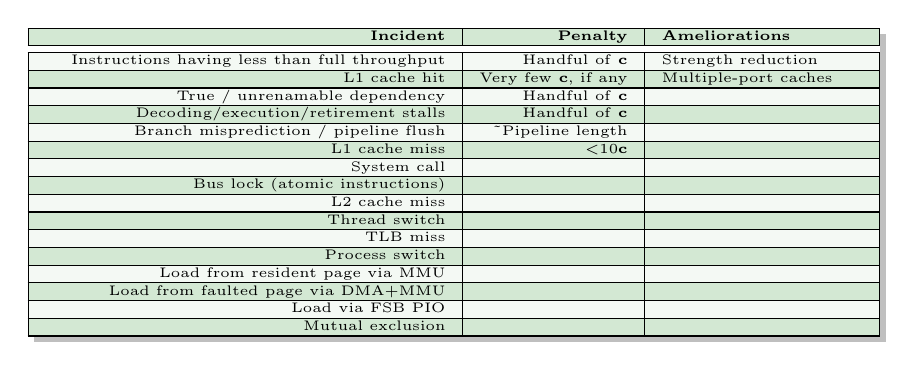
\begin{tikzpicture}
\node[drop shadow,fill=white,inner sep=0pt]
{\rowcolors{1}{ForestGreen!20}{ForestGreen!5}
{\tiny
\begin{tabular}{|>{\raggedleft}p{2in}|r|p{1in}|}
\hline
\textbf{Incident} & \textbf{Penalty} & \textbf{Ameliorations} \\
\hline\hline
Instructions having less than full throughput &
Handful of \textbf{c} &
Strength reduction \\
\hline
L1 cache hit & Very few \textbf{c}, if any & Multiple-port caches \\
\hline
True / unrenamable dependency & Handful of \textbf{c} & \\
\hline
Decoding/execution/retirement stalls & Handful of \textbf{c} & \\
\hline
Branch misprediction / pipeline flush & \textasciitilde Pipeline length & \\
\hline
L1 cache miss & <10\textbf{c} & \\
\hline
System call & & \\
\hline
Bus lock (atomic instructions) & & \\
\hline
L2 cache miss & & \\
\hline
Thread switch & & \\
\hline
TLB miss & & \\
\hline
Process switch & & \\
\hline
Load from resident page via MMU & & \\
\hline
Load from faulted page via DMA+MMU & & \\
\hline
Load via FSB PIO & & \\
\hline
Mutual exclusion & & \\
\hline
\end{tabular}%
}
};
\end{tikzpicture}
\end{center}
\end{frame}

\end{document}
